\documentclass[tikz,border=8pt]{standalone}
\usetikzlibrary{positioning,matrix}

\begin{document}

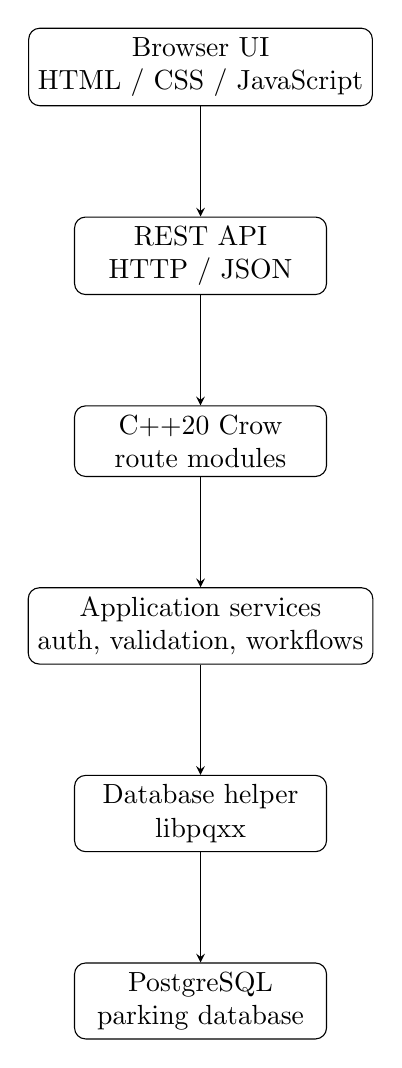
\begin{tikzpicture}[node distance=1.4cm, every node/.style={draw, rounded corners, align=center, minimum width=3.2cm, minimum height=0.8cm}, >=stealth]
  \node (ui) {Browser UI\\HTML / CSS / JavaScript};
  \node (api) [below=of ui] {REST API\\HTTP / JSON};
  \node (crow) [below=of api] {C++20 Crow\\route modules};
  \node (logic) [below=of crow] {Application services\\auth, validation, workflows};
  \node (db) [below=of logic] {Database helper\\libpqxx};
  \node (pg) [below=of db] {PostgreSQL\\parking database};
  \draw[->] (ui) -- (api);
  \draw[->] (api) -- (crow);
  \draw[->] (crow) -- (logic);
  \draw[->] (logic) -- (db);
  \draw[->] (db) -- (pg);
\end{tikzpicture}

\vspace{1cm}

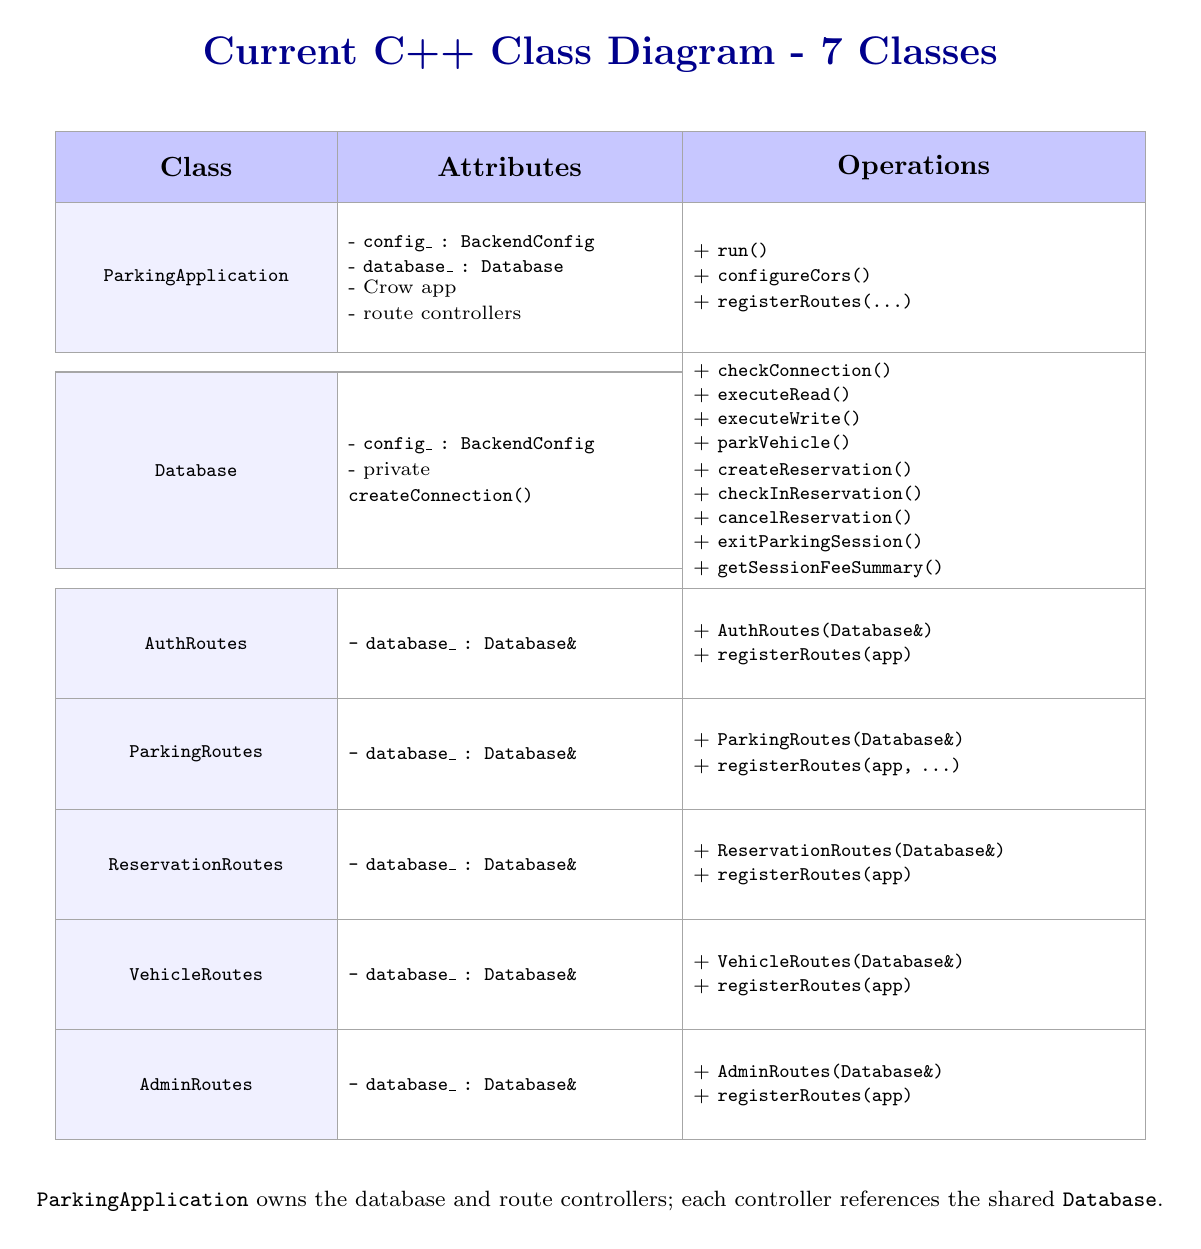
\begin{tikzpicture}[font=\small]
  \matrix (classTable) [
    matrix of nodes,
    nodes={draw=black!35, anchor=center, align=left, text width=5.6cm, inner sep=4pt, font=\scriptsize},
    column 1/.style={nodes={text width=3.3cm, align=center, fill=blue!6}},
    column 2/.style={nodes={text width=4.1cm}},
    column 3/.style={nodes={text width=5.6cm}},
    row 1/.style={nodes={fill=blue!22, font=\bfseries, align=center, minimum height=9mm}},
    row 2/.style={nodes={minimum height=19mm}},
    row 3/.style={nodes={minimum height=25mm}},
    row 4/.style={nodes={minimum height=14mm}},
    row 5/.style={nodes={minimum height=14mm}},
    row 6/.style={nodes={minimum height=14mm}},
    row 7/.style={nodes={minimum height=14mm}},
    row 8/.style={nodes={minimum height=14mm}},
    row sep=-\pgflinewidth,
    column sep=-\pgflinewidth
  ] {
    Class & Attributes & Operations \\
    \texttt{ParkingApplication} &
    \shortstack[l]{- \texttt{config\_ : BackendConfig}\\- \texttt{database\_ : Database}\\- Crow app\\- route controllers} &
    \shortstack[l]{+ \texttt{run()}\\+ \texttt{configureCors()}\\+ \texttt{registerRoutes(...)} } \\
    \texttt{Database} &
    \shortstack[l]{- \texttt{config\_ : BackendConfig}\\- private\\\texttt{createConnection()} } &
    \shortstack[l]{+ \texttt{checkConnection()}\\+ \texttt{executeRead()}\\+ \texttt{executeWrite()}\\+ \texttt{parkVehicle()}\\+ \texttt{createReservation()}\\+ \texttt{checkInReservation()}\\+ \texttt{cancelReservation()}\\+ \texttt{exitParkingSession()}\\+ \texttt{getSessionFeeSummary()} } \\
    \texttt{AuthRoutes} & \texttt{- database\_ : Database\&} & \shortstack[l]{+ \texttt{AuthRoutes(Database\&)}\\+ \texttt{registerRoutes(app)}} \\
    \texttt{ParkingRoutes} & \texttt{- database\_ : Database\&} & \shortstack[l]{+ \texttt{ParkingRoutes(Database\&)}\\+ \texttt{registerRoutes(app, ...)}} \\
    \texttt{ReservationRoutes} & \texttt{- database\_ : Database\&} & \shortstack[l]{+ \texttt{ReservationRoutes(Database\&)}\\+ \texttt{registerRoutes(app)}} \\
    \texttt{VehicleRoutes} & \texttt{- database\_ : Database\&} & \shortstack[l]{+ \texttt{VehicleRoutes(Database\&)}\\+ \texttt{registerRoutes(app)}} \\
    \texttt{AdminRoutes} & \texttt{- database\_ : Database\&} & \shortstack[l]{+ \texttt{AdminRoutes(Database\&)}\\+ \texttt{registerRoutes(app)}} \\
  };

  \node[above=5mm of classTable.north, font=\Large\bfseries, text=blue!55!black]
    {Current C++ Class Diagram - 7 Classes};
  \node[below=4mm of classTable.south, font=\footnotesize, align=center]
    {\texttt{ParkingApplication} owns the database and route controllers; each controller references the shared \texttt{Database}.};
\end{tikzpicture}

\end{document}
